\documentclass[dvipdfmx,twoside]{jsarticle}
\usepackage{amsmath,amssymb}
\usepackage{CJKutf8}
\usepackage{okumacro}
\usepackage{booktabs}
\usepackage{array}
\usepackage{xcolor}
\usepackage{colortbl}
\usepackage{tipa}
\usepackage{tikz}
\usepackage{fancybox}
\usepackage{wasysym}
\usepackage{pifont}
\usepackage{graphicx}
\usepackage{wrapfig}
\usepackage{geometry}
\geometry{margin=2cm}
\usepackage{fancyhdr}
\usepackage[utf8]{inputenc}
\usepackage{CJK}
% 设置页面样式
\pagestyle{fancy}
\fancyhf{}
\renewcommand{\headrulewidth}{0pt}
\fancyhead[RO]{数学–\thepage}
\fancyhead[LE]{数学–\thepage}

% 重新定义 plain 样式
\fancypagestyle{plain}{%
  \fancyhf{}%
  \renewcommand{\headrulewidth}{0pt}%
  \fancyhead[RO]{数学-\thepage}%
  \fancyhead[LE]{数学-\thepage}%
}
% 自定义A方框命令
\newcommand{\abb}[1]{%
\begin{tikzpicture}[baseline]
\node[draw=black, 
      rectangle, 
      minimum width=0.8cm, 
      minimum height=0.3cm, 
      fill=gray!25, 
      font=\bfseries,
      line width=1pt,
      inner sep=2pt,
      anchor=base] {#1};
\end{tikzpicture}%
}
\newcommand{\ab}[1]{%
\begin{tikzpicture}[baseline]
\node[draw=black, 
      rectangle, 
      minimum width=0.8cm, 
      minimum height=0.3cm, 
      font=\bfseries,
      line width=1pt,
      inner sep=2pt,
      anchor=base] {#1};
\end{tikzpicture}%
}

\newcommand{\maru}[1]{\tikz[baseline=-0.7ex]{
    \node[shape=circle,draw,inner sep=1pt,minimum size=5pt,anchor=center] {\footnotesize #1};}}
\definecolor{headercolor}{RGB}{220,220,220}
\definecolor{rowcolor1}{RGB}{245,245,245}
\definecolor{rowcolor2}{RGB}{255,255,255}

% \title{\vspace{-1.5cm} 2025年8月羚課文科数学月考 }
% \author{\textnosfal{Linc\ -\ 伊}}
\date{}
\begin{document}

\begin{CJK}{UTF8}{ipxm}  % 使用ipxm字体
  %月考表纸部分
\begin{center}

\vspace*{5cm}

% 学校logo

\includegraphics[width=5cm]{pics/1.jpg}

\vspace{2cm}

% 主标题
{\fontsize{24}{30}\selectfont\bfseries\sffamily
2025年9月\\
\vspace{1em}
羚課文科数学月考
}

\end{center}
\newpage
%第一部分
\noindent

\begin{tikzpicture}
\node[draw, rectangle, minimum width=1cm, minimum height=0.8cm, font=\Huge] {I};
\end{tikzpicture}
\\
\\
\textbf{問1}\qquad $y=-3(x-5)2-1$ のグラフは、$y=\ab{\color{red}{\textsf{AB}}} x^2$ のグラフを$x$軸の正の向きに $\ab{\color{red}{\textsf{C}}}$, y 軸の正の向きに\\[1em]
 $\ab{\color{red}{\textsf{DE}}}$ だけ平行移動したもので、頂点の座標は $ \left(\ab{\color{red}{\textsf{F}}}, \ab{\color{red}{\textsf{GH}}}\right) $である。
\\[20em]

\noindent
\textbf{問2}\qquad 二次関数$y=2x^2-12x+15$のグラフを点$(2,0)$に関して対称移動してできるグラフの方程式は\\[1em]
$y= \ab{\color{red}{\textsf{IJ}}} x^2- \ab{\color{red}{\textsf{K}}} x+ \ab{\color{red}{\textsf{L}}}$。
\newpage
\begin{center}
- 計算欄 (memo) -
\end{center}
\newpage
\noindent

\begin{tikzpicture}
\node[draw, rectangle, minimum width=1cm, minimum height=0.8cm, font=\Huge] {II};
\end{tikzpicture} 
\\
\\
\textbf{問1}\qquad 三個のサイコロを同時に投げる。このとき、\\

\noindent
(1)出る目の最小値が3以上になる確率は $\dfrac{\ab{\color{red}{\textsf{A}}}}{\ab{\color{red}{\textsf{BC}}}}$\\[0.5em]
(2)三個のサイコロのうち、いずれの二個の目の和が8になる確率は $\dfrac{\ab{\color{red}{\textsf{DE}}}}{\ab{\color{red}{\textsf{FG}}}}$\\[0.5em]
(3)出る目の最小値は2以下であり、かつどの二個の和も8でない場合の確率は $\dfrac{\ab{\color{red}{\textsf{EF}}}}{\ab{\color{red}{\textsf{GH}}}}$\\[10.5em]

\noindent
\textbf{問2}\qquad $a=\dfrac{4}{4-\sqrt{7}}$とする。$a$の分母を有理化すると\\[0.5em]

$$ a=\dfrac{\ab{\color{red}{\textsf{IJ}}}+\ab{\color{red}{\textsf{K}}}\sqrt{\ab{\color{red}{\textsf{L}}}}}{\ab{\color{red}{\textsf{M}}}} $$

\noindent
となる。\\

また、$r$を有理数とし、\\
$$ \beta = \dfrac{9-(r^2-3r)\sqrt{7}}{5} $$

\noindent
とする。\\

一般に,$\sqrt{7}$が無理数であることから、有理数$p$,$q$に対して、$p+q\sqrt{7}=0\Leftrightarrow\ p=q= \ab{\color{red}{\textsf{N}}}$
が成り立つ。\\
\newpage
\begin{center}
- 計算欄 (memo) -
\end{center}
\newpage
\noindent

\begin{tikzpicture}
\node[draw, rectangle, minimum width=1cm, minimum height=0.8cm, font=\Huge] {III};
\end{tikzpicture} 
\\
\\
\textbf{問1}\qquad (1) $\cos A=\dfrac{1}{3} (0\leq A \leq \pi)$のとき,$\tan A=\ab{\color{red}{\textsf{A}}}\sqrt{\ab{\color{red}{\textsf{B}}}}$\\[1em]

(2)$\alpha$が第2象限の角で、$\sin \alpha = \dfrac{3}{5}$のとき、次の値を求めよ。\\[0.5em]

$\sin 2\alpha = \dfrac{\ab{\color{red}{\textsf{CDE}}}}{FG}$, $\cos 2\alpha = \dfrac{\ab{\color{red}{\textsf{H}}}}{\ab{\color{red}{\textsf{IJ}}}}$,$\tan 2\alpha = \dfrac{\ab{\color{red}{\textsf{KLM}}}}{N}$\\[10em]

\textbf{問2}\qquad 三角形ABCにおいて、辺BCを7:1内分する点をDとし、辺ACを7:1内分する点をEとする。
線分ADと線分BEの交点をFとし、直線CFと辺ABの交点をGとする\\[0.5em]

このとき、
\[
\dfrac{\text{三角形}CDG\text{の面積}}{\text{三角形}BFG\text{の面積}} = \dfrac{\ab{\color{red}{\textsf{O}}}}{\ab{\color{red}{\textsf{PQ}}}}
\]
である。
四点$B, D, F, G$が同一円周上にあり、かつ$FD = 1$のとき
\[
AB = \ab{\color{red}{\textsf{RS}}}
\]
である。さらに、$AE = 3\sqrt{7}$とするとき、$AE:AC =\ab{\color{red}{\textsf{TU}}} $である。
\newpage
\begin{center}
- 計算欄 (memo) -
\end{center}
\newpage
\noindent

\begin{tikzpicture}
\node[draw, rectangle, minimum width=1cm, minimum height=0.8cm, font=\Huge] {IV};
\end{tikzpicture} 
\\
\\
\begin{minipage}[t]{0.5\textwidth}
\vspace{-4cm}
円 $O$ に内接する五角形 $ABCDE$ において

$AB = \sqrt{3}$, $BC = 4$, $DE = \sqrt{7}$,

$EA = 1$, $\angle EAB = 150°$

とする。このとき、円 $O$ の半径、辺 $CD$ の長さ、および、五角形 $ABCDE$ の面積を求めよう。
\end{minipage}
\hfill
\begin{minipage}[t]{0.45\textwidth}
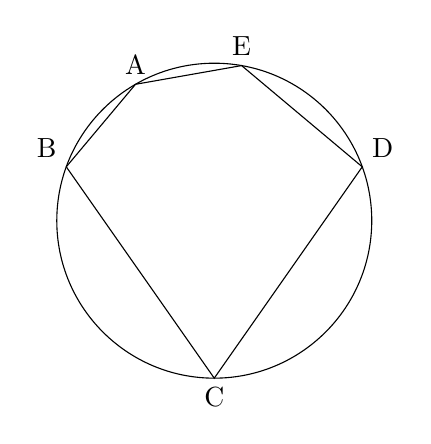
\begin{tikzpicture}[scale=0.8]
  % 定义圆心和半径
  \def\radius{2.5cm}
  \coordinate (O) at (0,0);

  % 绘制圆
  \draw (O) circle (\radius);

  % 定义并标记顶点
  \coordinate (E) at (80:\radius);
  \coordinate (D) at (20:\radius);
  \coordinate (C) at (-90:\radius);
  \coordinate (B) at (160:\radius);
  \coordinate (A) at (120:\radius);
  
  % 绘制多边形
  \draw (A) -- (B) -- (C) -- (D) -- (E) -- (A);

  % 在顶点旁边添加标签
  \node[above] at (E) {E};
  \node[above right] at (D) {D};
  \node[below] at (C) {C};
  \node[above left] at (B) {B};
  \node[above] at (A) {A};

\end{tikzpicture}
\end{minipage}

\noindent
(1) \quad $EB = \sqrt{\ab{\color{red}{\textsf{A}}}}$ であり、円 $O$ の半径は $\sqrt{\ab{\color{red}{\textsf{B}}}}$ である。\\[0.5em]

\noindent
(2) \quad $\angle BDE = \ab{\color{red}{\textsf{CD}}}°$ であるから、三角形 $BDE$ について、$\angle DEB = \ab{\color{red}{\textsf{EF}}G}°$ であり、

$BD = \sqrt{\ab{\color{red}{\textsf{HI}}}}$ である。\\[0.5em]

\noindent
(3) \quad $\angle BCD = \ab{\color{red}{\textsf{JK}}}°$ である。三角形 $BCD$ について、$CD = x$ とおいて余弦定理を用い

ると、$x$ の2次方程式\\[0.5em]

$$x^2 - \ab{\color{red}{\textsf{L}}}x - \ab{\color{red}{\textsf{M}}} = 0$$

を得る。$x > 0$ であるから\\[0.5em]

$$x = \ab{\color{red}{\textsf{N}}}$$

である。\\[0.5em]

\noindent
(4) \quad 五角形 $ABCDE$ の面積は $\ab{\color{red}{\textsf{O}}}\sqrt{\ab{\color{red}{\textsf{P}}}}$ である。
\end{CJK}
\end{document}